% !TEX program = xelatex
% 공통수학2 · Ⅰ. 도형의 방정식 · 2. 원의 방정식 · 01 원의 방정식 · 1/2차시
% 학생용 활동지 (답안 없음)
\documentclass[11pt,a4paper]{article}
\usepackage{kotex}
\usepackage{iftex}
\ifPDFTeX\else
  \setmainhangulfont{Noto Serif CJK KR}
  \setsanshangulfont{Noto Sans CJK KR}
\fi
\usepackage[margin=2.1cm]{geometry}
\usepackage{parskip}
\usepackage{enumitem}
\usepackage{array}
\usepackage{tabularx}
\usepackage{xcolor}
\usepackage{amssymb}
\usepackage{tikz}
\usepackage[most]{tcolorbox}
\usepackage{fancyhdr}
\usepackage{titlesec}

\definecolor{goldc}{HTML}{B07C22}
\definecolor{goldstrong}{HTML}{8A5F16}
\definecolor{indigoc}{HTML}{2B3B57}
\definecolor{indigosoft}{HTML}{6E82A6}
\definecolor{linec}{HTML}{D6DACB}
\definecolor{surface2}{HTML}{E4E8DC}
\definecolor{writeline}{HTML}{C7CCBA}
\definecolor{inksoft}{HTML}{52604F}

\titleformat{\section}{\normalfont\sffamily\bfseries\large\color{indigoc}}{\thesection}{0.6em}{}
\titlespacing{\section}{0pt}{14pt}{6pt}
\newtcolorbox{goalbox}{enhanced, breakable, colback=white, colframe=goldc, boxrule=0.5pt, leftrule=3pt, arc=2pt, left=10pt, right=10pt, top=8pt, bottom=8pt}
\newtcolorbox{sheetbox}{enhanced, breakable, colback=white, colframe=linec, boxrule=0.6pt, arc=3pt, left=11pt, right=11pt, top=9pt, bottom=9pt}
\newcommand{\writespace}[1]{%
  \par\nobreak\vspace{3pt}
  \foreach \n in {1,...,#1} {%
    \noindent\textcolor{writeline}{\rule{\linewidth}{0.4pt}}\par\vspace{0.62cm}%
  }
}
\newcommand{\fillblank}[1]{\makebox[#1]{\hrulefill}}
\pagestyle{fancy}\fancyhf{}\renewcommand{\headrulewidth}{0pt}
\fancyfoot[L]{\footnotesize\color{inksoft} 공통수학2 · 2026학년도 2학기 · 지평선고등학교}
\fancyfoot[R]{\footnotesize\color{inksoft} 다음 시간 --- 01 원의 방정식(2) 일반형}

\begin{document}

\noindent
\begin{minipage}[b]{0.62\linewidth}
  {\sffamily\footnotesize\color{indigosoft} 공통수학2 · Ⅰ. 도형의 방정식 · 2. 원의 방정식}\\[2pt]
  {\sffamily\bfseries\Large 01 원의 방정식 \textperiodcentered\ 9차시}
\end{minipage}\hfill
\begin{minipage}[b]{0.36\linewidth}
  \raggedleft\small\color{inksoft}
  반\ \fillblank{1.6cm} \quad 번호\ \fillblank{1.6cm}\\[4pt]
  이름\ \fillblank{3.6cm}
\end{minipage}

\vspace{4pt}
\noindent{\color{goldc}\rule{\linewidth}{2.2pt}}
\vspace{10pt}

\begin{goalbox}
\textbf{오늘의 목표}\\
원의 정의로부터 원의 방정식을 유도하고, 중심과 반지름 (또는 지름의 양 끝 점)이 주어졌을 때 원의 방정식을 구할 수 있다.
\vspace{4pt}
\small\color{inksoft}
$\square$ 자신 있음 \quad $\square$ 조금 헷갈림 \quad $\square$ 처음 봄 \hfill (수업 전 나의 상태에 표시)
\end{goalbox}

\section{생각 열기 --- 원형 관개 농업}

\begin{sheetbox}
반지름의 길이가 $10$인 원 모양의 문양을 중심이 원점 O와 일치하도록 좌표평면 위에 나타냈다. 문양의 가장자리의 한 점을 P$(x,y)$라 하자.

\begin{center}
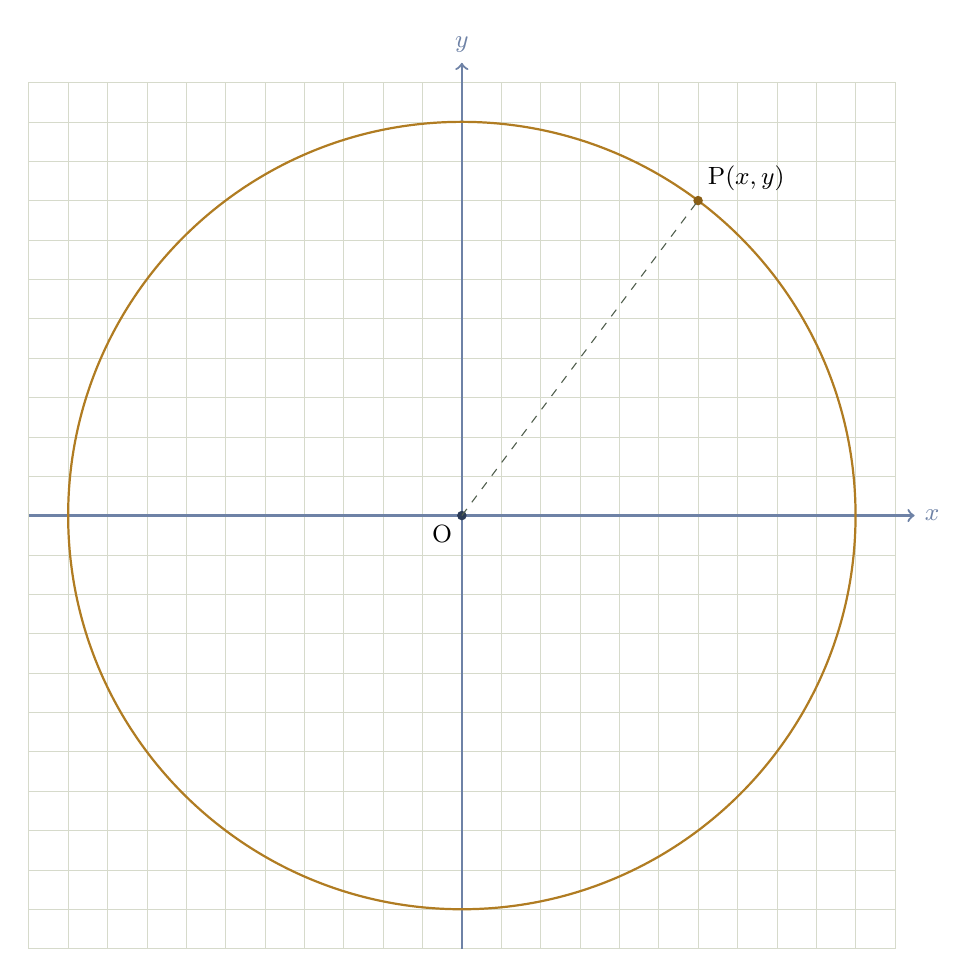
\begin{tikzpicture}[scale=0.5]
  \draw[step=1cm, linec, very thin] (-11,-11) grid (11,11);
  \draw[->, thick, indigosoft] (-11,0) -- (11.5,0) node[right, font=\small]{$x$};
  \draw[->, thick, indigosoft] (0,-11) -- (0,11.5) node[above, font=\small]{$y$};
  \draw[thick, goldc] (0,0) circle (10);
  \filldraw[indigoc] (0,0) circle (3pt);
  \node[below left, font=\small] at (0,0) {O};
  \filldraw[goldstrong] (6,8) circle (3pt);
  \node[above right, font=\small] at (6,8) {P$(x,y)$};
  \draw[dashed, inksoft] (0,0) -- (6,8);
\end{tikzpicture}
\end{center}

$\overline{\text{OP}}=10$임을 이용하여 다음 식을 완성해 보자.
\[
x^2+y^2 = \fillblank{3cm}
\]
\end{sheetbox}

\section{개념 정리 --- 원의 방정식}

\begin{sheetbox}
중심 C$(a,b)$, 반지름 $r$인 원 위의 점을 P$(x,y)$라 하면 $\overline{\text{CP}}=r$이므로
\[
\sqrt{\fillblank{5cm}} = r
\]
양변을 제곱하여 정리하면

\[
\boxed{(x-a)^2+(y-b)^2 = \fillblank{1.6cm}}
\]

특히, 중심이 원점이고 반지름이 $r$인 원의 방정식은 $\fillblank{3cm}$

\vspace{8pt}
\textbf{보기} --- 중심$(2,-1)$, 반지름 $3$인 원: $(x-2)^2+(y+1)^2=\fillblank{1.6cm}$
\end{sheetbox}

\section{연습 문제}

\begin{sheetbox}
\textbf{1.} 다음 원의 방정식을 구하시오.\\
\hspace*{1.6em}⑴ 중심의 좌표가 $(-3,0)$이고 반지름의 길이가 $2$인 원\\
\hspace*{1.6em}⑵ 중심이 원점이고 점 $(3,-4)$를 지나는 원
\writespace{3}

\vspace{8pt}
\textbf{2.} 두 점 A$(-4,10)$과 B$(8,-6)$을 지름의 양 끝 점으로 하는 원의 방정식을 구하시오. (힌트: 중심 = 중점, 반지름 = 중심에서 한 점까지 거리)
\writespace{4}
\end{sheetbox}

\section{사고의 가시화 --- See · Think · Wonder}

\noindent{\footnotesize\color{inksoft} 오늘 배운 `원의 방정식'을 떠올리며 아래 세 칸을 채워 보자.}\\[6pt]
\begin{tabularx}{\linewidth}{@{}XXX@{}}
\textbf{\footnotesize\color{indigoc} See --- 무엇을 보았나?} &
\textbf{\footnotesize\color{indigoc} Think --- 무엇을 생각했나?} &
\textbf{\footnotesize\color{indigoc} Wonder --- 무엇이 궁금한가?} \\[4pt]
\end{tabularx}
\noindent
\begin{minipage}[t]{0.32\linewidth}\writespace{3}\end{minipage}\hfill
\begin{minipage}[t]{0.32\linewidth}\writespace{3}\end{minipage}\hfill
\begin{minipage}[t]{0.32\linewidth}\writespace{3}\end{minipage}

\section{마무리 성찰}

\begin{sheetbox}
\begin{minipage}[t]{0.48\linewidth}
{\footnotesize\color{inksoft} 오늘 배운 것을 한 문장으로}
\writespace{2}
\end{minipage}\hfill
\begin{minipage}[t]{0.48\linewidth}
{\footnotesize\color{inksoft} 감사 일기 / 유념 한 줄}
\writespace{2}
\end{minipage}
\end{sheetbox}

\end{document}
